% Strongly Connected Components -- Metropolis beamer slides
% Compile: pdflatex strongly-connected-components.tex (x2)
\documentclass[10pt,aspectratio=169]{beamer}

\usetheme{metropolis}
\metroset{block=fill, numbering=fraction, progressbar=frametitle}

\usepackage[T1]{fontenc}
\usepackage{amsmath, amssymb}
\usepackage{listings}
\usepackage{booktabs}
\usepackage{tikz}
\usetikzlibrary{arrows.meta, positioning, calc}

% ---- colors -------------------------------------------------------------
\definecolor{mLightBlue}{HTML}{4C72B0}
\definecolor{mGreen}{HTML}{55A868}
\definecolor{mRed}{HTML}{C44E52}
\definecolor{mGray}{HTML}{BFBFBF}
\definecolor{mOrange}{HTML}{DD8452}
\setbeamercolor{alerted text}{fg=mRed}

% ---- code style ---------------------------------------------------------
\lstdefinestyle{jl}{
  basicstyle=\ttfamily\footnotesize,
  keywordstyle=\color{mRed}\bfseries,
  commentstyle=\color{mGreen}\itshape,
  numberstyle=\tiny\color{mGray},
  showstringspaces=false,
  breaklines=true,
  columns=fullflexible,
  morekeywords={function,for,in,if,else,elseif,end,return,length,while}
}
\lstset{style=jl}

% ---- graph helpers ------------------------------------------------------
\tikzset{
  vtx/.style={draw, circle, minimum size=6.5mm, inner sep=0pt, font=\small,
              fill=white},
  edg/.style={thick, mGray!80!black},
  dedg/.style={edg, -{Stealth[length=2.3mm]}},
  tree/.style={line width=1.8pt, black},
  sccbox/.style={draw=mGray!70!black, dashed, rounded corners=8pt},
  scclbl/.style={font=\small},
  cmp/.style={draw, rounded corners=3pt, minimum width=12mm,
              minimum height=7mm, font=\small},
  % fills for the four components; frames switch them on as needed
  gA/.style={}, gB/.style={}, gC/.style={}, gD/.style={},
  fillA/.style={gA/.style={fill=mLightBlue!35}},
  fillB/.style={gB/.style={fill=mGreen!35}},
  fillC/.style={gC/.style={fill=mOrange!40}},
  fillD/.style={gD/.style={fill=mRed!30}},
  fillall/.style={fillA, fillB, fillC, fillD},
}

% The running example. #1 = 0 draws G, 1 draws its transpose G^T.
% #2 = 1 draws the DFS tree edges of the first pass in bold.
% Per-vertex options can be added with the style v<i> (e.g. v13/.style=...).
\newcommand{\sccgraph}[2]{%
  \foreach \i/\x/\y/\g in {1/0/1.3/A, 2/1.2/0.8/A, 3/1.2/-0.8/A, 4/0/-1.3/A,
      5/-1.2/0/A, 6/3.0/1.0/B, 7/5.0/1.5/B, 8/5.0/-1.5/B, 9/3.0/-1.0/B,
      10/7.6/0.7/C, 11/7.6/-0.7/C, 12/10.2/0/D, 13/11.0/0.9/D, 14/11.0/-0.9/D}
    \node[vtx, g\g, v\i/.try] (v\i) at (\x,\y) {\i};
  \foreach \a/\b/\o/\t in {1/2/0/1, 2/3/0/1, 3/4/0/1, 4/2/0/0, 4/5/0/1,
      5/1/0/0, 6/7/0/1, 7/8/0/1, 8/6/0/0, 8/9/0/1, 9/6/0/0, 10/11/25/1,
      11/10/25/0, 12/13/25/0, 13/14/25/1, 14/12/25/1, 5/6/-20/1, 9/10/0/1,
      11/13/-20/1, 2/9/0/0, 7/12/30/0} {
    \ifnum#2=1 \ifnum\t=1 \def\es{tree}\else\def\es{}\fi \else\def\es{}\fi
    \ifnum#1=0
      \draw[dedg, \es] (v\a) to[bend left=\o] (v\b);
    \else
      \draw[dedg] (v\b) to[bend right=\o] (v\a);
    \fi
  }
}
\newcommand{\sccboxes}{%
  \draw[sccbox] (-1.75,-1.85) rectangle (1.75,1.85);
  \draw[sccbox] (2.45,-2.05) rectangle (5.55,2.05);
  \draw[sccbox] (7.0,-1.3) rectangle (8.2,1.3);
  \draw[sccbox] (9.6,-1.5) rectangle (11.6,1.5);
  \node[scclbl] at (0,2.15) {$A$};
  \node[scclbl] at (4.0,2.35) {$B$};
  \node[scclbl] at (7.6,-1.6) {$C$};
  \node[scclbl] at (10.6,1.8) {$D$};
}

% ---- title --------------------------------------------------------------
\title{Strongly Connected Components}
\subtitle{Two Passes of DFS}
\date{}
\author{}

\begin{document}

\maketitle

% =========================================================================
\begin{frame}{From Undirected to Directed}
  In an \alert{undirected} graph, one DFS per unvisited vertex finds the
  connected components: if $u$ reaches $v$, then $v$ reaches $u$.

  \pause
  \bigskip
  In a \alert{directed} graph that symmetry is gone.

  \bigskip
  \begin{center}
  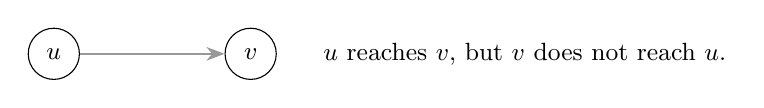
\begin{tikzpicture}[scale=1.0, every node/.style={transform shape}]
    \node[vtx] (u) at (0,0) {$u$}; \node[vtx] (v) at (2.5,0) {$v$};
    \draw[dedg] (u) -- (v);
    \node[right] at (3.3,0) {\small $u$ reaches $v$, but $v$ does not reach $u$.};
  \end{tikzpicture}
  \end{center}

  \pause
  \bigskip
  \begin{center}
    So what is the right notion of a ``component'' for directed graphs?
  \end{center}
\end{frame}

\begin{frame}{Strongly Connected Components}
  \begin{block}{Definition}
    A \alert{strongly connected component (SCC)} of a directed graph is a
    maximal set $S \subseteq V$ such that for every $u, v \in S$ there is a
    path from $u$ to $v$ \alert{and} a path from $v$ to $u$.
  \end{block}

  \begin{center}
  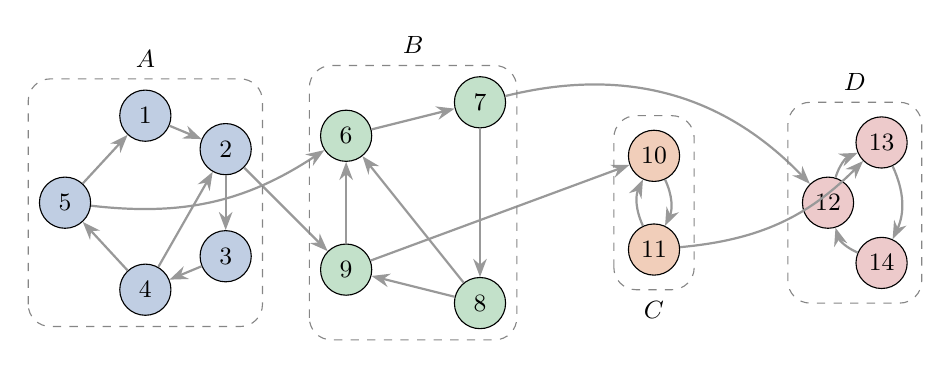
\begin{tikzpicture}[scale=0.85, fillall]
    \sccgraph{0}{0}
    \sccboxes
  \end{tikzpicture}
  \end{center}

  \begin{center}
    \small Four SCCs: $A = \{1,\ldots,5\}$, $B = \{6,\ldots,9\}$,
    $C = \{10, 11\}$, $D = \{12, 13, 14\}$.
  \end{center}
\end{frame}

% =========================================================================
\section{The Contracted Graph}

\begin{frame}{Contract Each SCC}
  Shrink every SCC to a single vertex, keeping an edge $X \to Y$ whenever some
  edge of $G$ goes from $X$ to $Y$.

  \bigskip
  \begin{center}
  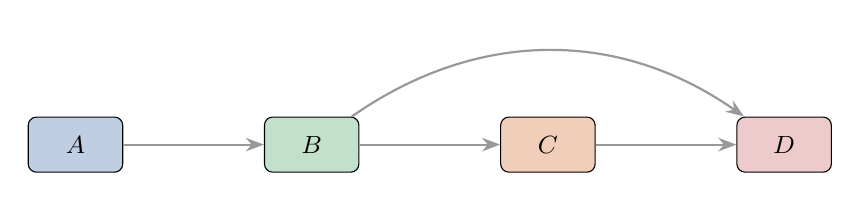
\begin{tikzpicture}[scale=1.0]
    \node[cmp, fill=mLightBlue!35] (A) at (0,0) {$A$};
    \node[cmp, fill=mGreen!35]     (B) at (3,0) {$B$};
    \node[cmp, fill=mOrange!40]    (C) at (6,0) {$C$};
    \node[cmp, fill=mRed!30]       (D) at (9,0) {$D$};
    \draw[dedg] (A) -- (B); \draw[dedg] (B) -- (C); \draw[dedg] (C) -- (D);
    \draw[dedg] (B) to[bend left=35] (D);
  \end{tikzpicture}
  \end{center}

  \pause
  \bigskip
  \begin{block}{Observation 1}
    The contracted graph is always a \alert{DAG}.
  \end{block}
\end{frame}

\begin{frame}{Why a DAG?}
  Suppose the contracted graph had a cycle
  \[
    X_1 \to X_2 \to \cdots \to X_k \to X_1 .
  \]

  \pause
  \begin{itemize}
    \item Inside each $X_i$, every vertex reaches every other.
    \item Following the cycle, every vertex of $X_1$ reaches every vertex of
          $X_k$, and every vertex of $X_k$ reaches every vertex of $X_1$.
  \end{itemize}

  \pause
  \bigskip
  So $X_1 \cup \cdots \cup X_k$ is strongly connected, contradicting the
  \alert{maximality} of each $X_i$. $\square$
\end{frame}

\begin{frame}{Sources and Sinks}
  \begin{itemize}
    \item A \alert{source} SCC has no edges coming in from other SCCs.
    \item A \alert{sink} SCC has no edges going out to other SCCs.
  \end{itemize}

  \bigskip
  \begin{center}
  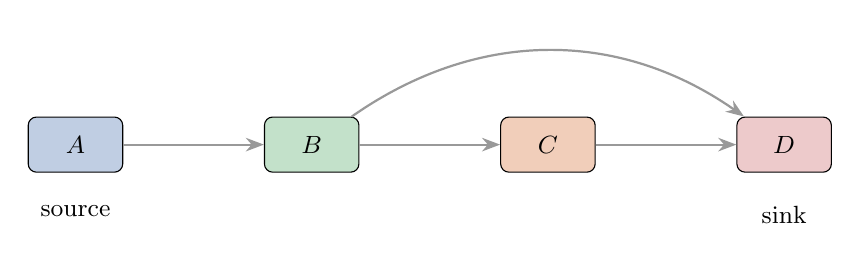
\begin{tikzpicture}[scale=1.0]
    \node[cmp, fill=mLightBlue!35] (A) at (0,0) {$A$};
    \node[cmp, fill=mGreen!35]     (B) at (3,0) {$B$};
    \node[cmp, fill=mOrange!40]    (C) at (6,0) {$C$};
    \node[cmp, fill=mRed!30]       (D) at (9,0) {$D$};
    \draw[dedg] (A) -- (B); \draw[dedg] (B) -- (C); \draw[dedg] (C) -- (D);
    \draw[dedg] (B) to[bend left=35] (D);
    \node[below=3mm of A, font=\small] {source};
    \node[below=3mm of D, font=\small] {sink};
  \end{tikzpicture}
  \end{center}

  \bigskip
  \begin{center}
    Every DAG has at least one source and one sink, and may have several.
  \end{center}
\end{frame}

% =========================================================================
\section{Finding a Sink}

\begin{frame}{The Idea}
  Run DFS from a vertex in a \alert{sink} SCC. No edge leaves the sink, so
  DFS visits \alert{exactly} that SCC.

  \begin{center}
  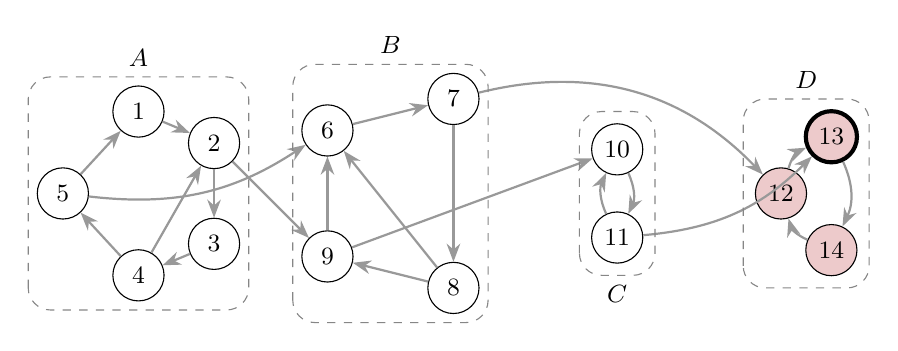
\begin{tikzpicture}[scale=0.8, fillD, v13/.style={line width=1.5pt}]
    \sccgraph{0}{0}
    \sccboxes
  \end{tikzpicture}
  \end{center}

  \begin{center}
    \small DFS from $13$ visits $13, 14, 12$: exactly $D$.
  \end{center}

  \pause
  \begin{center}
    Then delete $D$ and repeat on what remains.
    \alert{But how do we find a vertex in a sink without knowing the SCCs?}
  \end{center}
\end{frame}

\begin{frame}{Post Numbers Point the Way}
  \begin{block}{Observation 2}
    If there is an edge from SCC $X$ to SCC $Y$ (so $X$ comes before $Y$ in
    the DAG), then
    \[
      \max_{v \in X} post[v] \;>\; \max_{w \in Y} post[w].
    \]
  \end{block}

  \bigskip
  By transitivity the same holds whenever $X$ reaches $Y$ in the contracted
  DAG.

  \pause
  \bigskip
  \begin{center}
    So the vertex with the \alert{largest} post number lies in a
    \alert{source} SCC.
  \end{center}
\end{frame}

\begin{frame}{Proof of Observation 2}
  Let $z$ be the first vertex of $X \cup Y$ that DFS visits.

  \pause
  \bigskip
  \textbf{Case 1: $z \in X$.} When $z$ is visited, all of $X \cup Y$ is
  unvisited, and $z$ reaches every vertex of $X \cup Y$. So DFS visits all of
  them before $z$ finishes:
  \[
    post[z] > post[w] \quad\text{for every } w \in Y.
  \]

  \pause
  \textbf{Case 2: $z \in Y$.} Since $X$ reaches $Y$ and the contracted graph
  is a DAG, $Y$ \alert{cannot} reach $X$. So \texttt{visit(z)} finishes all of
  $Y$ without touching $X$, and every vertex of $X$ is visited, and finishes,
  later.

  \pause
  \bigskip
  In both cases $\max_X post > \max_Y post$. $\square$

  \bigskip
  \small Careful: in case 1 only $z$ is guaranteed to beat all of $Y$. Other
  vertices of $X$ may finish early.
\end{frame}

\begin{frame}{Example: pre/post Numbers}
  DFS on $G$ from vertex $1$, neighbours in increasing order. Bold edges form
  the DFS tree.

  \bigskip
  \begin{center}
  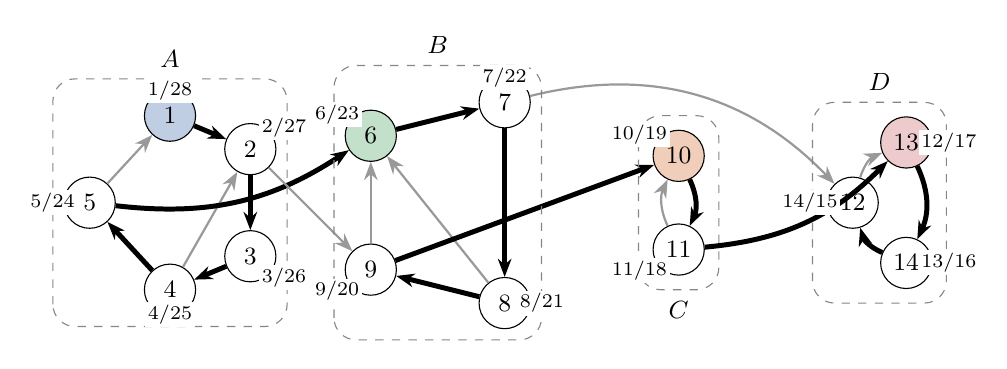
\begin{tikzpicture}[scale=0.85,
      lab/.style={font=\scriptsize, inner sep=1pt, fill=white},
      gA/.style={}, v1/.style={fill=mLightBlue!35}, v6/.style={fill=mGreen!35},
      v10/.style={fill=mOrange!40}, v13/.style={fill=mRed!30}]
    \sccgraph{0}{1}
    \sccboxes
    \foreach \i/\a/\b/\pos in {1/1/28/above, 2/2/27/above right,
        3/3/26/below right, 4/4/25/below, 5/5/24/left,
        6/6/23/above left, 7/7/22/above, 8/8/21/right,
        9/9/20/below left, 10/10/19/above left,
        11/11/18/below left, 12/14/15/left, 13/12/17/right,
        14/13/16/right}
      \node[lab, \pos=1.5mm] at (v\i) {\a/\b};
  \end{tikzpicture}
  \end{center}

  \begin{center}
    \small Highest post number per SCC: $A$: $28$, $B$: $23$, $C$: $19$,
    $D$: $17$. They decrease along the DAG $A \to B \to C \to D$.
  \end{center}
\end{frame}

\begin{frame}{Flip the Edges}
  The largest post number finds a \alert{source}, but we want a \alert{sink}.

  \pause
  \bigskip
  \begin{block}{Observation 3}
    The \alert{transpose} $G^T$ (every edge reversed) has the same SCCs as
    $G$, and its contracted DAG is $G$'s with every edge reversed. So the
    sources of $G$ are exactly the sinks of $G^T$.
  \end{block}

  \begin{center}
  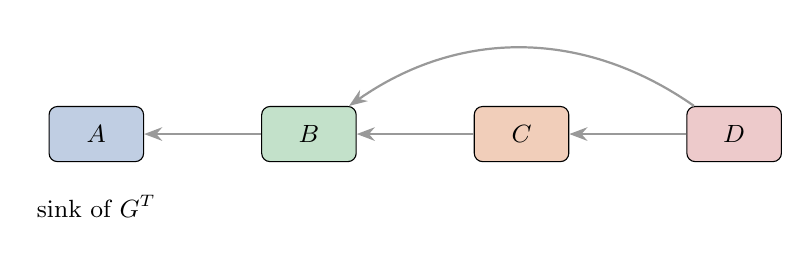
\begin{tikzpicture}[scale=0.9]
    \node[cmp, fill=mLightBlue!35] (A) at (0,0) {$A$};
    \node[cmp, fill=mGreen!35]     (B) at (3,0) {$B$};
    \node[cmp, fill=mOrange!40]    (C) at (6,0) {$C$};
    \node[cmp, fill=mRed!30]       (D) at (9,0) {$D$};
    \draw[dedg] (B) -- (A); \draw[dedg] (C) -- (B); \draw[dedg] (D) -- (C);
    \draw[dedg] (D) to[bend right=35] (B);
    \node[below=3mm of A, font=\small] {sink of $G^T$};
  \end{tikzpicture}
  \end{center}

  \bigskip
  \begin{center}
    \small $u$ and $v$ reach each other in $G$ $\iff$ they do in $G^T$:
    just reverse both paths.
  \end{center}
\end{frame}

% =========================================================================
\section{The Algorithm}

\begin{frame}{Two Passes of DFS}
  \begin{enumerate}
    \item Run DFS on $G$ and record post numbers.
    \bigskip
    \item Run DFS on $G^T$, starting new searches in \alert{decreasing} order
          of post number. Each DFS tree of this pass is one SCC.
  \end{enumerate}

  \pause
  \bigskip
  \textbf{Why it works.} The first start is the vertex with the largest post
  number, which lies in a source of $G$, so in a \alert{sink} of $G^T$. Its
  DFS collects exactly that SCC.

  \pause
  \bigskip
  After those vertices are marked, the next unvisited vertex with the largest
  post number lies in a source of what remains of $G$ (Observation 2 still
  applies to the remaining SCCs), hence in a sink of what remains of $G^T$.
  Repeat.
\end{frame}

\begin{frame}{Second Pass on $G^T$}
  Starts in decreasing post order: $1\ (28)$, then $6\ (23)$, $10\ (19)$,
  $13\ (17)$.

  \bigskip
  \begin{center}
  \begin{tikzpicture}[scale=0.85,
      fillA/.style={}, fillB/.style={}, fillC/.style={}, fillD/.style={}]
    \only<2->{\tikzset{gA/.style={fill=mLightBlue!35}}}
    \only<3->{\tikzset{gB/.style={fill=mGreen!35}}}
    \only<4->{\tikzset{gC/.style={fill=mOrange!40}}}
    \only<5->{\tikzset{gD/.style={fill=mRed!30}}}
    \sccgraph{1}{0}
    \sccboxes
  \end{tikzpicture}
  \end{center}

  \begin{center}
    \small
    \only<1>{The graph $G^T$: every edge of $G$ reversed.}%
    \only<2>{DFS from $1$ on $G^T$ reaches only $\{1,2,3,4,5\}$: SCC $A$.}%
    \only<3>{DFS from $6$ reaches $\{6,7,8,9\}$; edge $6 \to 5$ hits a visited
             vertex. SCC $B$.}%
    \only<4>{DFS from $10$ reaches $\{10, 11\}$: SCC $C$.}%
    \only<5>{DFS from $13$ reaches $\{13, 12, 14\}$: SCC $D$. Done.}
  \end{center}
\end{frame}

\begin{frame}{Running Time}
  \begin{itemize}
    \item First DFS on $G$: $O(n + m)$.
    \item Build $G^T$: one pass over the adjacency lists, $O(n + m)$.
    \item Second DFS on $G^T$: $O(n + m)$. Sorting by post number is free:
          just record vertices in the order they finish and read the list
          backwards.
  \end{itemize}

  \bigskip
  \begin{alertblock}{}
    \centering All SCCs in $O(n + m)$ time.
  \end{alertblock}
\end{frame}

\begin{frame}[fragile]{In Julia: First Pass}
\begin{lstlisting}[basicstyle=\ttfamily\scriptsize]
function strongly_connected_components(n, adj)
    # Step 1: DFS on G, recording vertices as they finish
    visited = falses(n)
    post_order = Int[]
    function dfs1(v)
        visited[v] = true
        for w in adj[v]
            if !visited[w]
                dfs1(w)
            end
        end
        push!(post_order, v)          # v finishes
    end
    for v in 1:n
        if !visited[v]
            dfs1(v)
        end
    end
\end{lstlisting}
\end{frame}

\begin{frame}[fragile]{In Julia: Transpose}
  Reverse every edge: $u \to v$ in $G$ becomes $v \to u$ in $G^T$.

  \bigskip
\begin{lstlisting}
    # Step 2: build the transpose G^T
    adj_t = [Int[] for _ in 1:n]
    for u in 1:n
        for v in adj[u]
            push!(adj_t[v], u)
        end
    end
\end{lstlisting}

  \bigskip
  \begin{center}
    One pass over all adjacency lists: $O(n + m)$.
  \end{center}
\end{frame}

\begin{frame}[fragile]{In Julia: Second Pass}
\begin{lstlisting}[basicstyle=\ttfamily\scriptsize]
    # Step 3: DFS on G^T in decreasing post order
    fill!(visited, false)
    scc_id = zeros(Int, n)
    num_scc = 0
    function dfs2(v, id)
        visited[v] = true
        scc_id[v] = id
        for w in adj_t[v]
            if !visited[w]
                dfs2(w, id)
            end
        end
    end
    for v in reverse(post_order)      # largest post number first
        if !visited[v]
            num_scc += 1
            dfs2(v, num_scc)
        end
    end
    return num_scc, scc_id
end
\end{lstlisting}
\end{frame}

% ---------------------------------------------------------------- exercise
\begin{frame}{Exercise}
  \begin{center}
    Run the algorithm on this graph (neighbours in increasing order, first
    pass starting from $1$). Give the post numbers and the SCCs in the order
    they are found.
  \end{center}

  \bigskip
  \begin{center}
  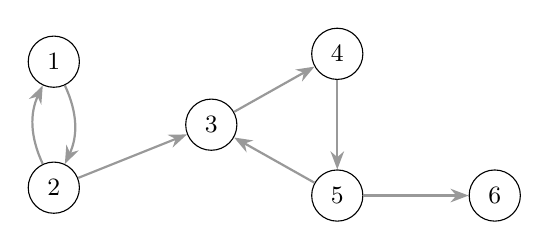
\begin{tikzpicture}[scale=1.0]
    \node[vtx] (1) at (0,0.8) {1};  \node[vtx] (2) at (0,-0.8) {2};
    \node[vtx] (3) at (2,0) {3};    \node[vtx] (4) at (3.6,0.9) {4};
    \node[vtx] (5) at (3.6,-0.9) {5}; \node[vtx] (6) at (5.6,-0.9) {6};
    \draw[dedg] (1) to[bend left=25] (2); \draw[dedg] (2) to[bend left=25] (1);
    \draw[dedg] (2) -- (3); \draw[dedg] (3) -- (4); \draw[dedg] (4) -- (5);
    \draw[dedg] (5) -- (3); \draw[dedg] (5) -- (6);
  \end{tikzpicture}
  \end{center}
\end{frame}

\begin{frame}{Solution}
  \textbf{First pass on $G$.} $1 \to 2 \to 3 \to 4 \to 5 \to 6$, then
  everything unwinds:
  \begin{center}
  \begin{tabular}{lcccccc}
    \toprule
    vertex & 1 & 2 & 3 & 4 & 5 & 6 \\
    \midrule
    pre/post & 1/12 & 2/11 & 3/10 & 4/9 & 5/8 & 6/7 \\
    \bottomrule
  \end{tabular}
  \end{center}

  \pause
  \bigskip
  \textbf{Second pass on $G^T$}, in order $1, 2, 3, 4, 5, 6$:
  \begin{itemize}
    \item from $1$: $\{1, 2\}$ (in $G^T$, $2 \to 3$ is reversed, so $3$ is
          not reached);
    \item from $3$: $\{3, 5, 4\}$;
    \item from $6$: $\{6\}$, since its only edge in $G^T$ goes to $5$, already
          visited.
  \end{itemize}

  \bigskip
  \begin{center}
    Three SCCs: $\{1,2\}$, $\{3,4,5\}$, $\{6\}$.
  \end{center}
\end{frame}

\end{document}
